%! Author = kyoto
%! Date = 11.09.2023

\vspace{3cm}
\tableofcontents

\newpage

\section{Текст задания.}
\begin{enumerate}
    \item На основе предложенной предметной области (текста) составить ее описание. Из полученного описания выделить сущности, их атрибуты и связи.
    \item Составить инфологическую модель.
    \item Составить даталогическую модель. При описании типов данных для атрибутов должны использоваться типы из СУБД PostgreSQL.
    \item Реализовать даталогическую модель в PostgreSQL. При описании и реализации даталогической модели должны учитываться ограничения целостности, которые характерны для полученной предметной области.
    \item Заполнить созданные таблицы тестовыми данными.
\end{enumerate}

\section{Описание предметной области.}
В сопровождении Элли и Малкольма, Грант обошел главное здание. Следом за ними шел мальчик. Грант любил детей. А как их
можно не любить, когда они так непосредственно, так страстно интересуются динозаврами. Гранту приходилось видеть, как в
музеях дети стояли с открытыми ртами, взирая на огромные скелеты, уходящие под самый потолок. Он часто спрашивал себя,
поче- му вымершие ящеры производят такое сильное впечатление на детей. Но потом он понял, что дети любят динозавров
потому, что эти гигантские создания воплощают в себе управляемую силу неограниченной власти. Динозавры символизируют
родителей, которых дети обожают, но боятся. Дети любят динозавров точно так же, как они любят своих родителей.

несколько людей могут ходить вокруг главного здания. люди могут преследовать друг друга.

\section{Список и классификация сущностей.}

\subsection{Стержневые.}
\begin{enumerate}
    \item actors
    \item actions
    \item feels
\end{enumerate}

\subsection{Ассоциативные.}

\begin{enumerate}
    \item events
    \item expressions
\end{enumerate}

\subsection{Характеристические.}

\begin{enumerate}
    \item groups
\end{enumerate}

\section{Инфологическая модель.}
\begin{figure}[H]
	\centering
	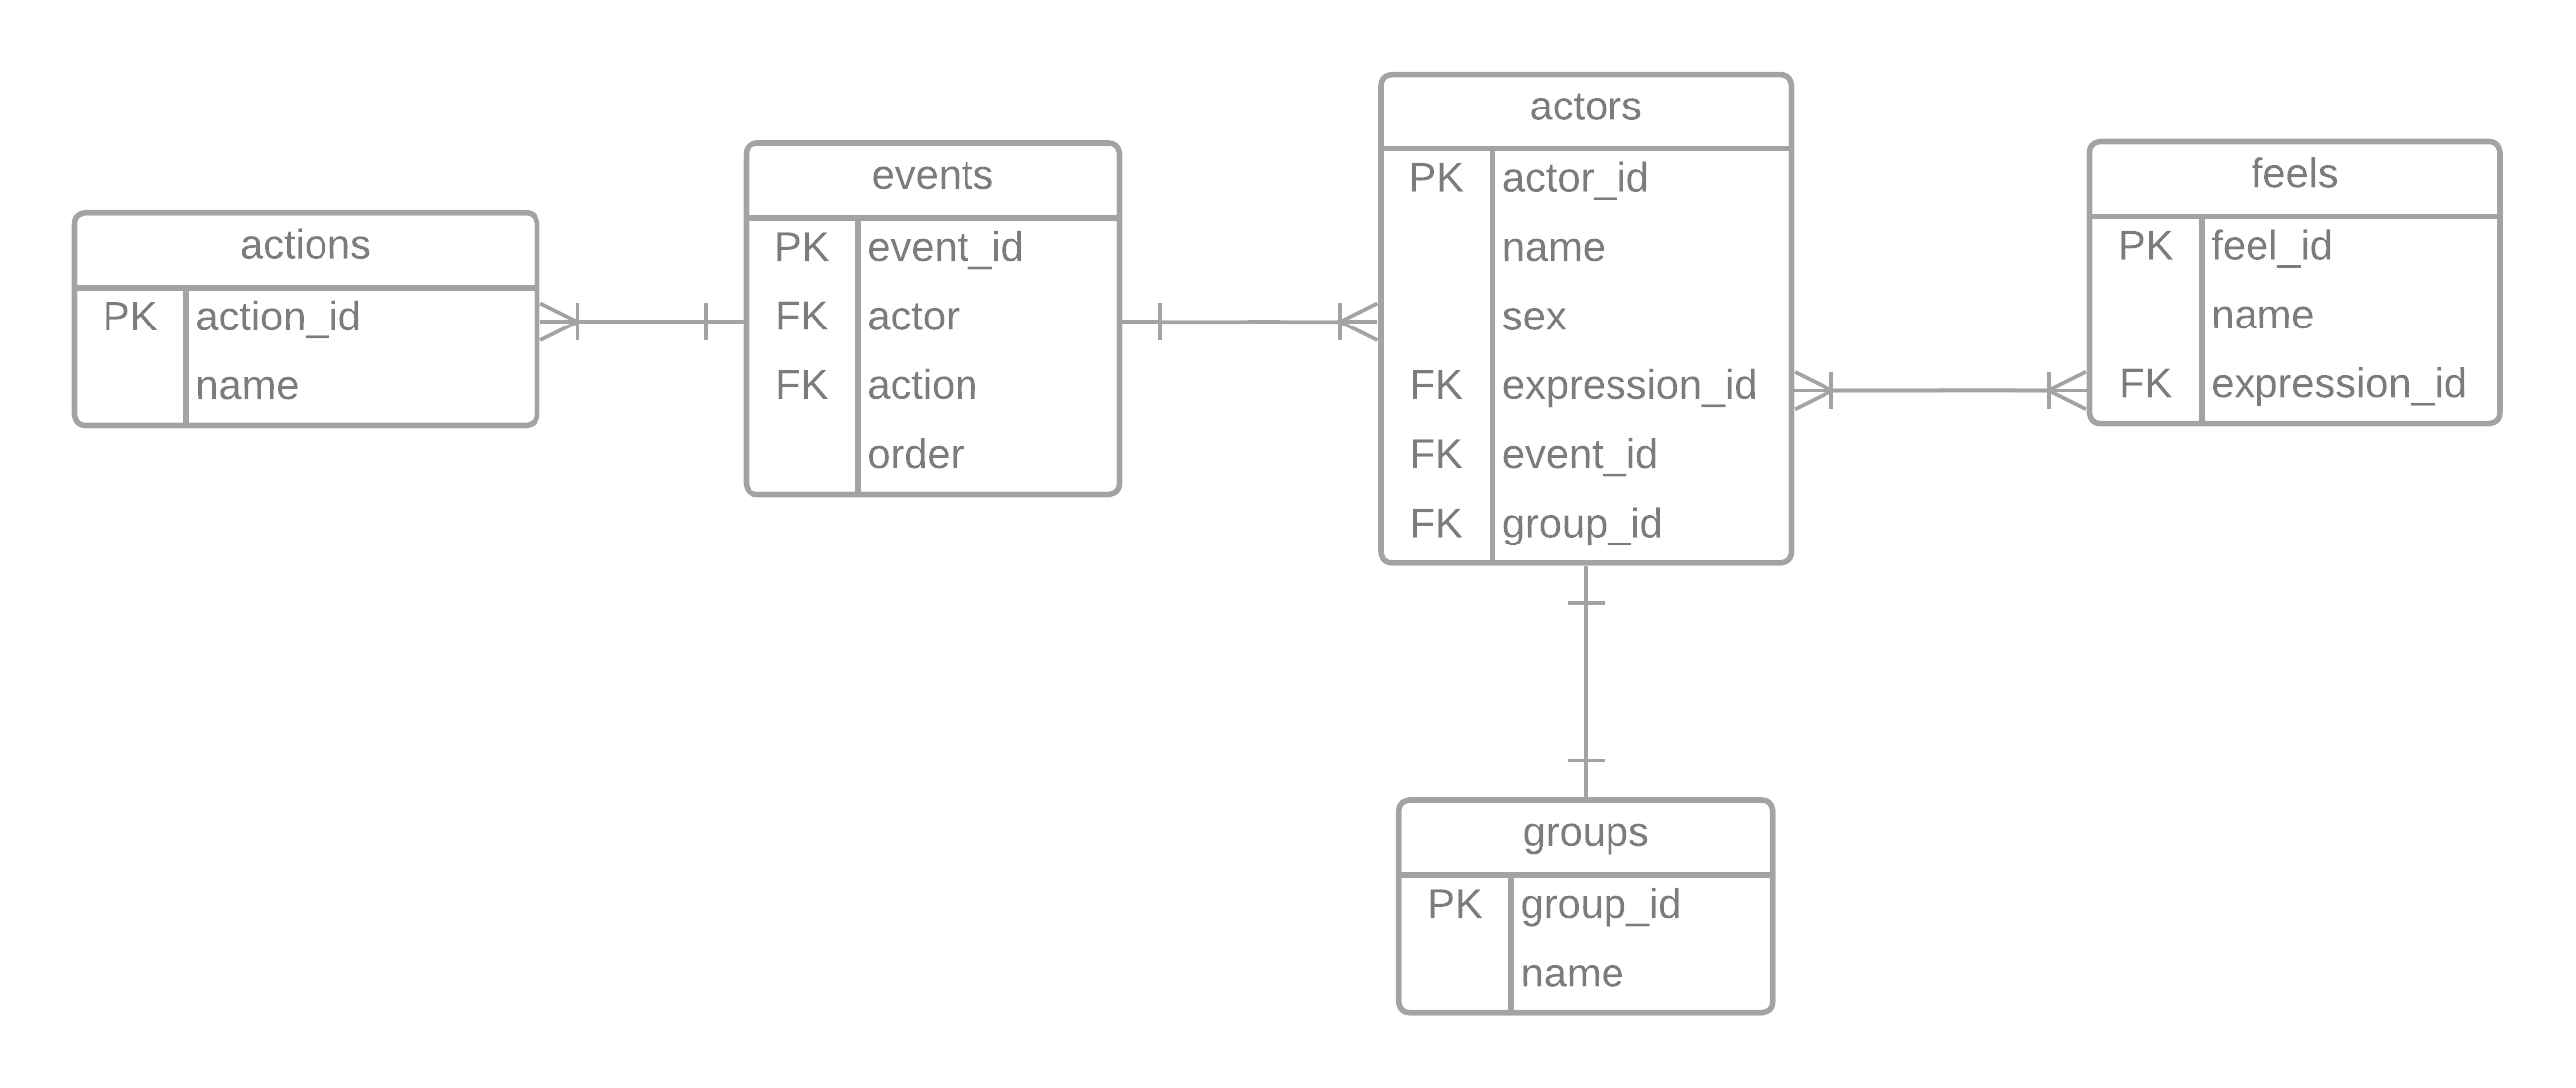
\includegraphics[scale=0.15]{img/info_model}
\end{figure}

\section{Даталогическая модель.}
\begin{figure}[H]
	\centering
	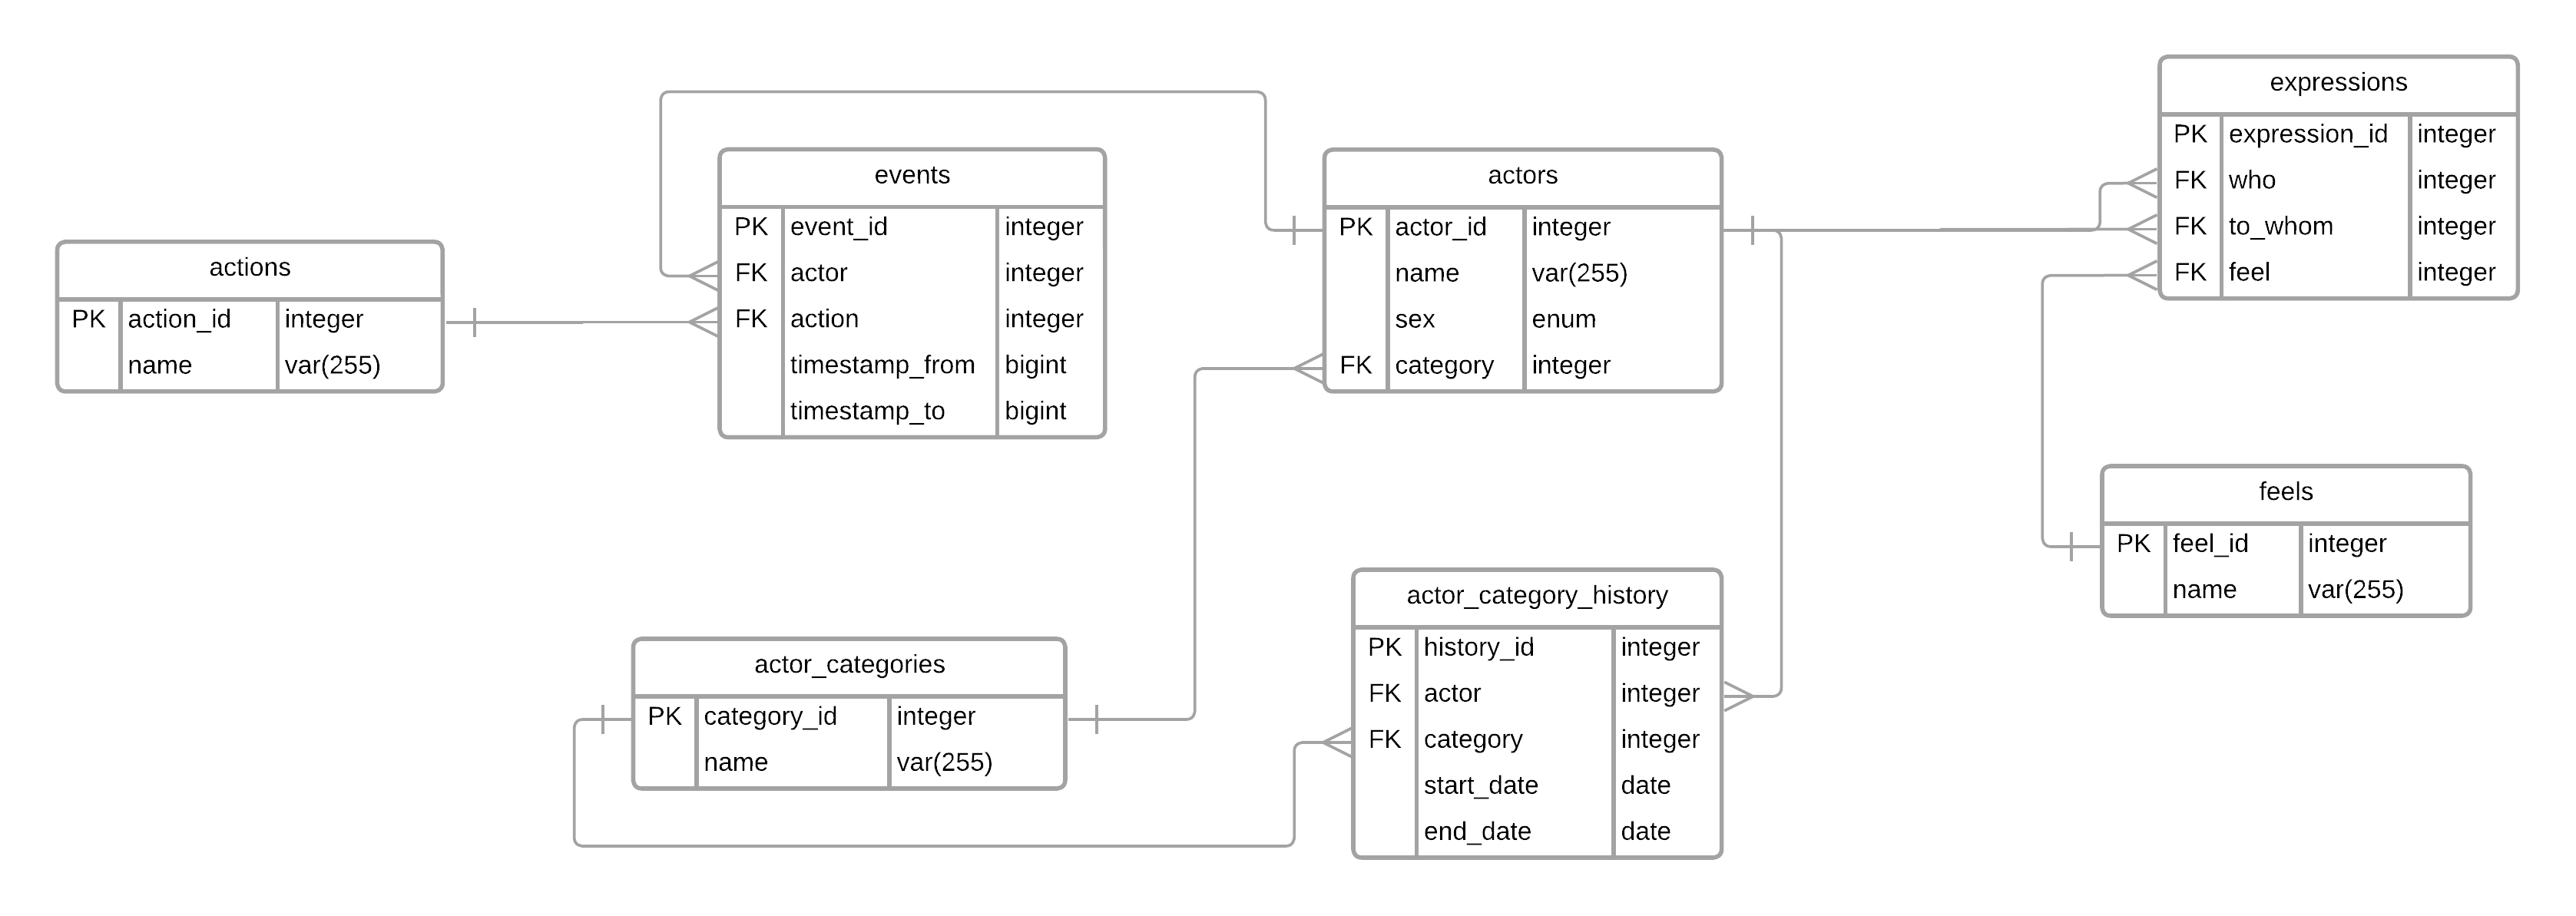
\includegraphics[scale=0.25]{img/data_model}
\end{figure}

\newpage

\section{Реализация даталогической модели на SQL.}
\tiny
%! Author = kyoto
%! Date = 12.09.2023
\begin{verbatim}
CREATE TYPE sex AS ENUM ('male', 'female', 'both');

CREATE TABLE actions (
    action_id SERIAL PRIMARY KEY,
    name VARCHAR(255) NOT NULL
);

CREATE TABLE feels (
    feel_id SERIAL PRIMARY KEY,
    name VARCHAR(255) NOT NULL
);

CREATE TABLE actor_categories (
    category_id SERIAL PRIMARY KEY,
    name VARCHAR(255) NOT NULL
);


CREATE TABLE actors (
    actor_id SERIAL PRIMARY KEY,
    name VARCHAR(255),
    sex sex,
    category INT REFERENCES actor_categories(category_id)
);

CREATE TABLE actor_category_history (
    history_id SERIAL PRIMARY KEY,
    actor INT NOT NULL,
    category INT NOT NULL,
    start_date DATE,
    end_date DATE,
    FOREIGN KEY (actor) REFERENCES actors(actor_id),
    FOREIGN KEY (category) REFERENCES actor_categories(category_id)
);

CREATE TABLE events (
    event_id SERIAL PRIMARY KEY,
    actor INT REFERENCES actors(actor_id) NOT NULL,
    action INT REFERENCES actions(action_id) NOT NULL,
    timestamp_from BIGINT,
    timestamp_to BIGINT
);

CREATE TABLE expressions (
    expression_id SERIAL PRIMARY KEY,
    who INT REFERENCES actors(actor_id) NOT NULL,
    to_whom INT REFERENCES actors(actor_id) NOT NULL,
    feel INT REFERENCES feels(feel_id) NOT NULL
);
\end{verbatim}
%! Author = kyoto
%! Date = 12.09.2023

\begin{verbatim}
INSERT INTO groups (name)
VALUES
    ('взрослые'),
    ('дети'),
    ('родители'),
    ('экспонаты');

INSERT INTO actors (name, sex, group_id)
VALUES
    ('элли', 'female', (SELECT group_id FROM groups WHERE name = 'взрослые')),
    ('малкольм', 'male', (SELECT group_id FROM groups WHERE name = 'взрослые')),
    ('грант', 'male', (SELECT group_id FROM groups WHERE name = 'взрослые')),
    ('мальчик', 'male', (SELECT group_id FROM groups WHERE name = 'дети')),
    ('дети', 'both', (SELECT group_id FROM groups WHERE name = 'дети')),
    ('родители', 'both', (SELECT group_id FROM groups WHERE name = 'родители')),
    ('динозавры', 'both', (SELECT group_id FROM groups WHERE name = 'экспонаты'));

INSERT INTO feels (name)
VALUES
    ('любовь'),
    ('интерес'),
    ('производить впечатление'),
    ('обожание'),
    ('страх');

INSERT INTO actions (name)
VALUES
    ('обойти здание'),
    ('следовать'),
    ('смотреть'),
    ('стоять');


INSERT INTO expressions (who, to_whom, feel)
VALUES
    ((SELECT actor_id FROM actors WHERE name = 'грант'), (SELECT actor_id FROM actors WHERE name = 'дети'), (SELECT feel_id FROM feels WHERE name = 'любовь')),
    ((SELECT actor_id FROM actors WHERE name = 'дети'), (SELECT actor_id FROM actors WHERE name = 'динозавры'), (SELECT feel_id FROM feels WHERE name = 'интерес')),
    ((SELECT actor_id FROM actors WHERE name = 'динозавры'), (SELECT actor_id FROM actors WHERE name = 'дети'), (SELECT feel_id FROM feels WHERE name = 'производить впечатление')),
    ((SELECT actor_id FROM actors WHERE name = 'дети'), (SELECT actor_id FROM actors WHERE name = 'динозавры'), (SELECT feel_id FROM feels WHERE name = 'любовь')),
    ((SELECT actor_id FROM actors WHERE name = 'дети'), (SELECT actor_id FROM actors WHERE name = 'родители'), (SELECT feel_id FROM feels WHERE name = 'обожание')),
    ((SELECT actor_id FROM actors WHERE name = 'дети'), (SELECT actor_id FROM actors WHERE name = 'родители'), (SELECT feel_id FROM feels WHERE name = 'страх')),
    ((SELECT actor_id FROM actors WHERE name = 'дети'), (SELECT actor_id FROM actors WHERE name = 'родители'), (SELECT feel_id FROM feels WHERE name = 'любовь'));

INSERT INTO events (actor, action, order_or)
VALUES
    ((SELECT actor_id FROM actors WHERE name = 'элли'), (SELECT action_id FROM actions WHERE name = 'обойти здание'), 1),
    ((SELECT actor_id FROM actors WHERE name = 'малкольм'), (SELECT action_id FROM actions WHERE name = 'обойти здание'), 1),
    ((SELECT actor_id FROM actors WHERE name = 'грант'), (SELECT action_id FROM actions WHERE name = 'обойти здание'), 1),
    ((SELECT actor_id FROM actors WHERE name = 'мальчик'), (SELECT action_id FROM actions WHERE name = 'следовать'), 2),
    ((SELECT actor_id FROM actors WHERE name = 'дети'), (SELECT action_id FROM actions WHERE name = 'стоять'), 3),
    ((SELECT actor_id FROM actors WHERE name = 'дети'), (SELECT action_id FROM actions WHERE name = 'смотреть'), 4);
\end{verbatim}
\normalsize

\newpage

\section{Выводы по работе.}
В результате выполнения лабораторной работы были применены навыки выявления
сущностей по описанию предметной области, создана инфологическая и даталогическая
модель, получены навыки написания DDL и DML запросов на языке SQL для базы данных
PostgreSQL.